\documentclass[a4paper]{article}
\usepackage{polski}
\usepackage[utf8]{inputenc}
\usepackage{enumerate}
\usepackage{graphicx}
\usepackage{float}

\usepackage{geometry}
\newgeometry{tmargin=2.5cm, bmargin=2cm, lmargin=2cm, rmargin=2cm}

\title{Założenia projektowe, specyfikacja funkcjonalna, kryteria ewaluacji}
\date{}
\author{}

\begin{document}
\maketitle



\section{Dekompozycja układu mechanicznego i elektronicznego:} 
\begin{figure}[H]
\centering
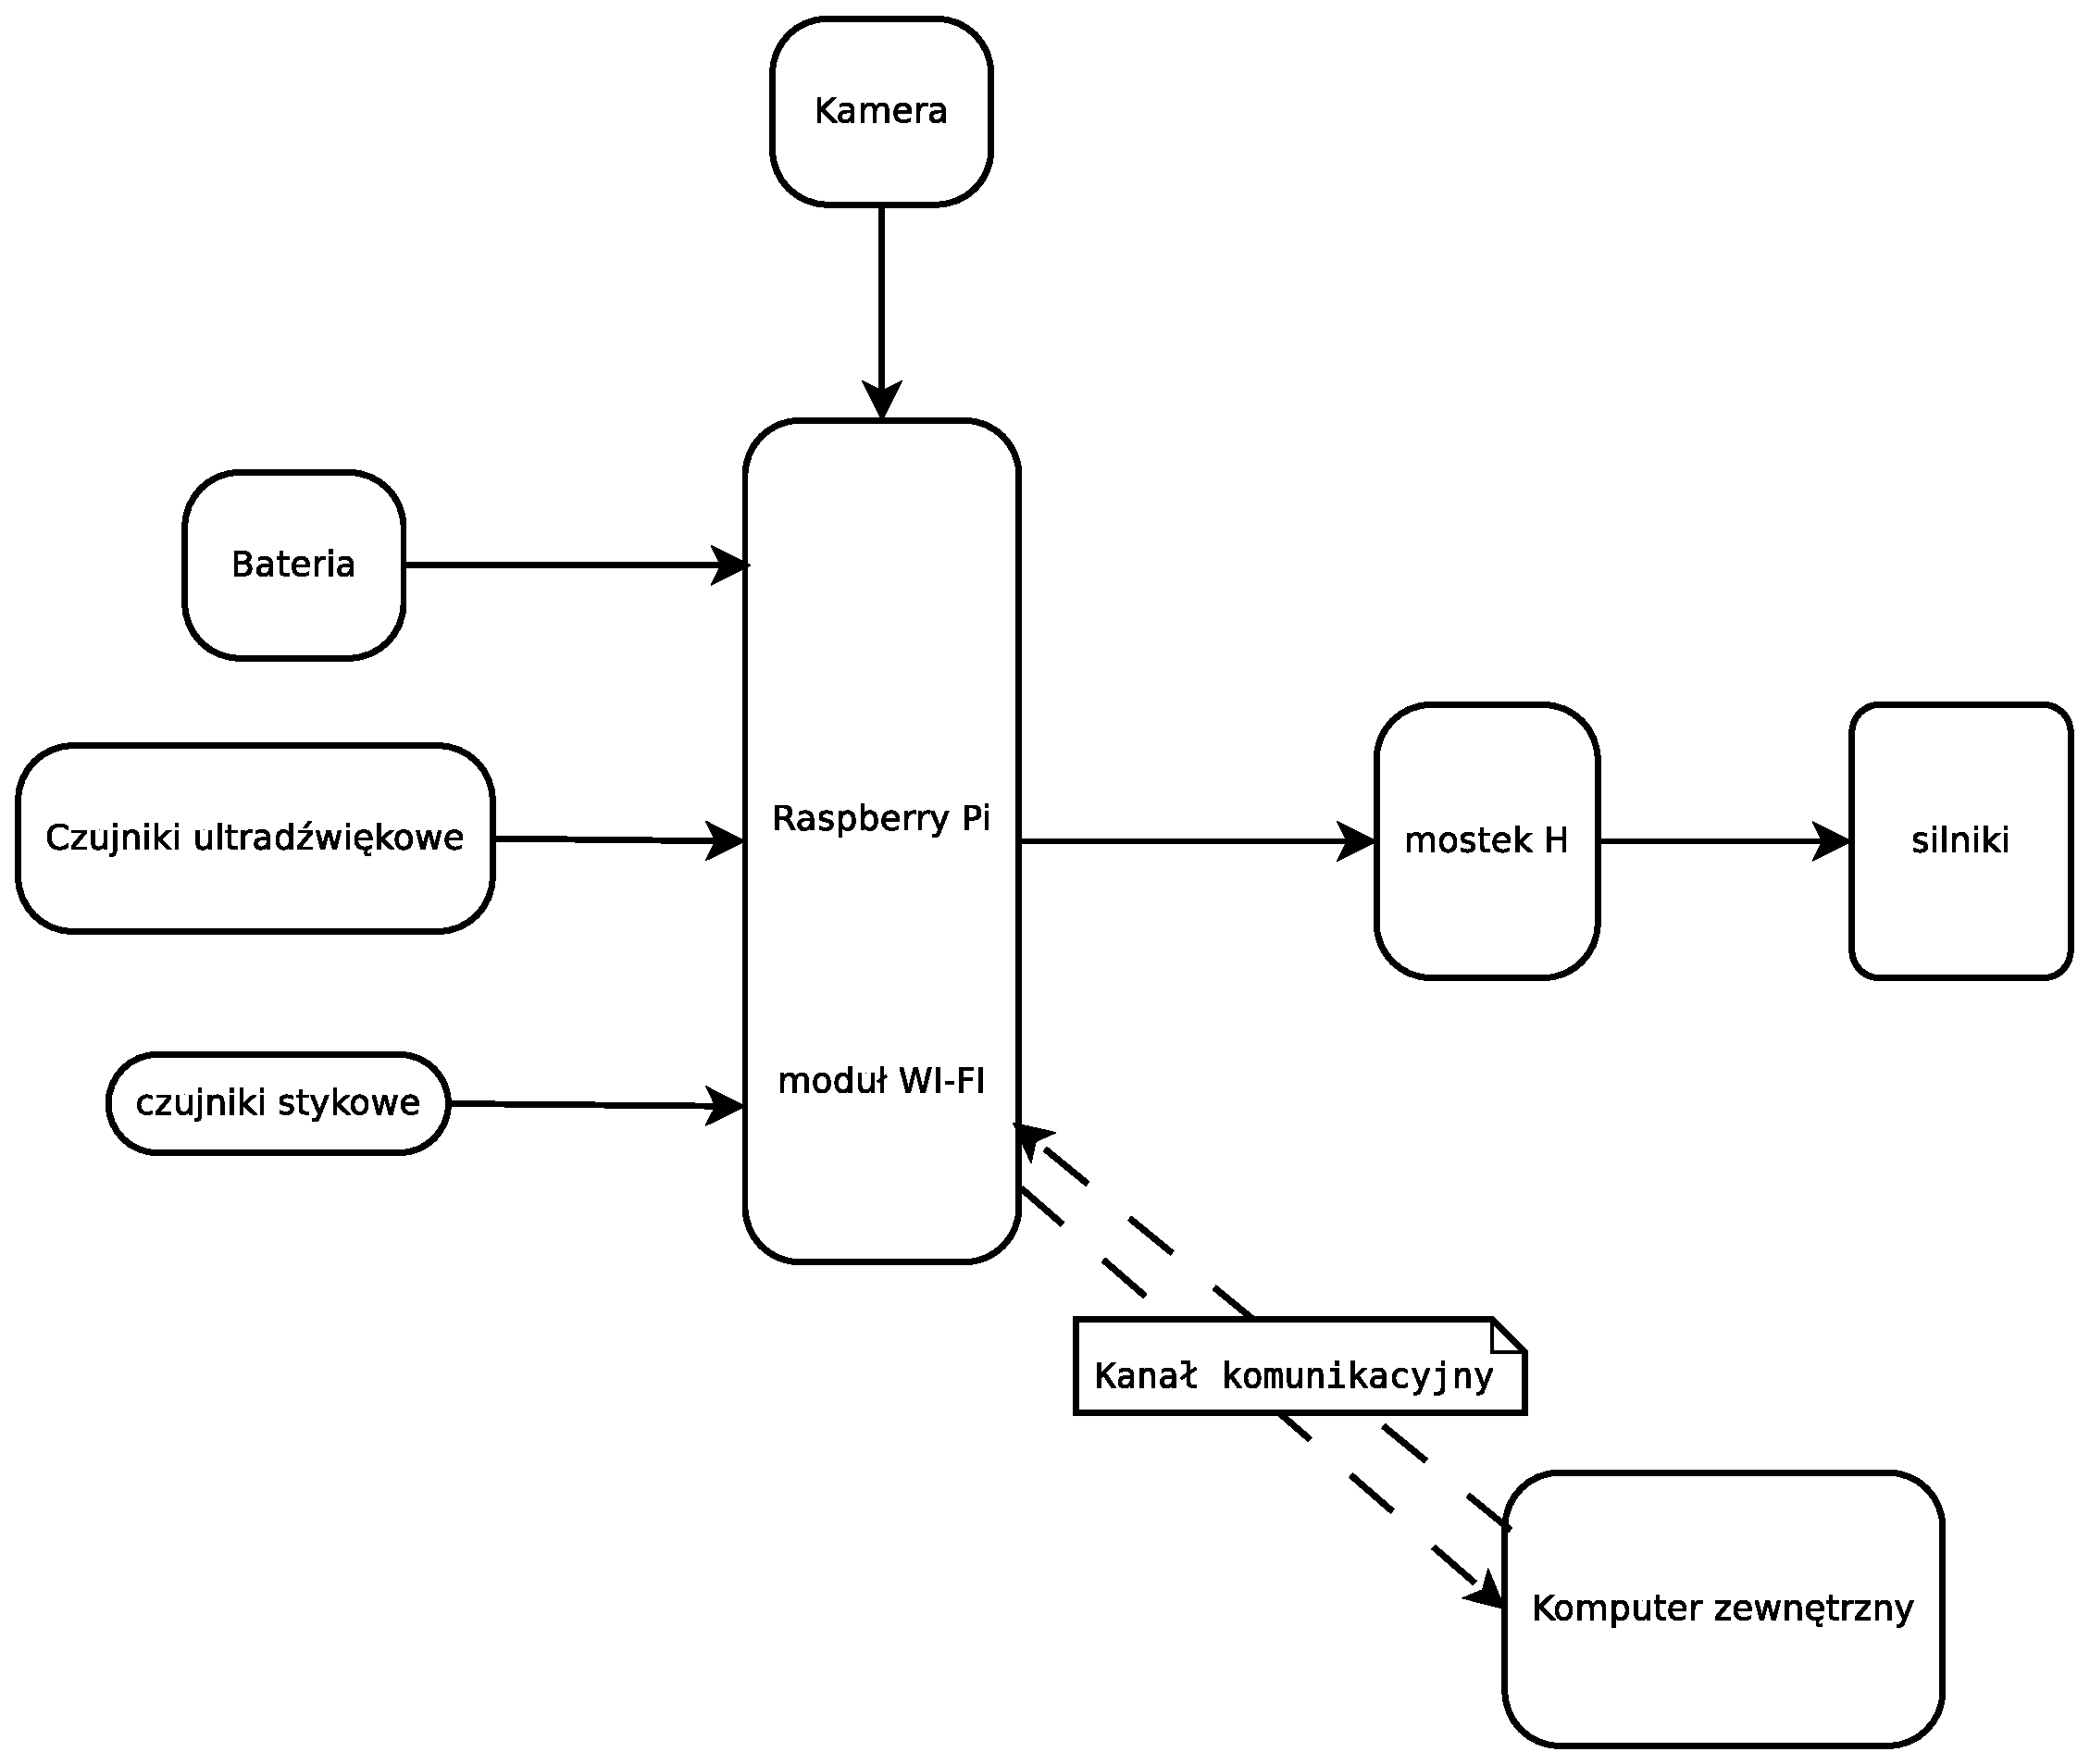
\includegraphics[width=15cm]{idea_sprzet-mech.eps}
\end{figure}

\section{Dekompozycja oprogramowania:}
\begin{figure}[H]
\centering
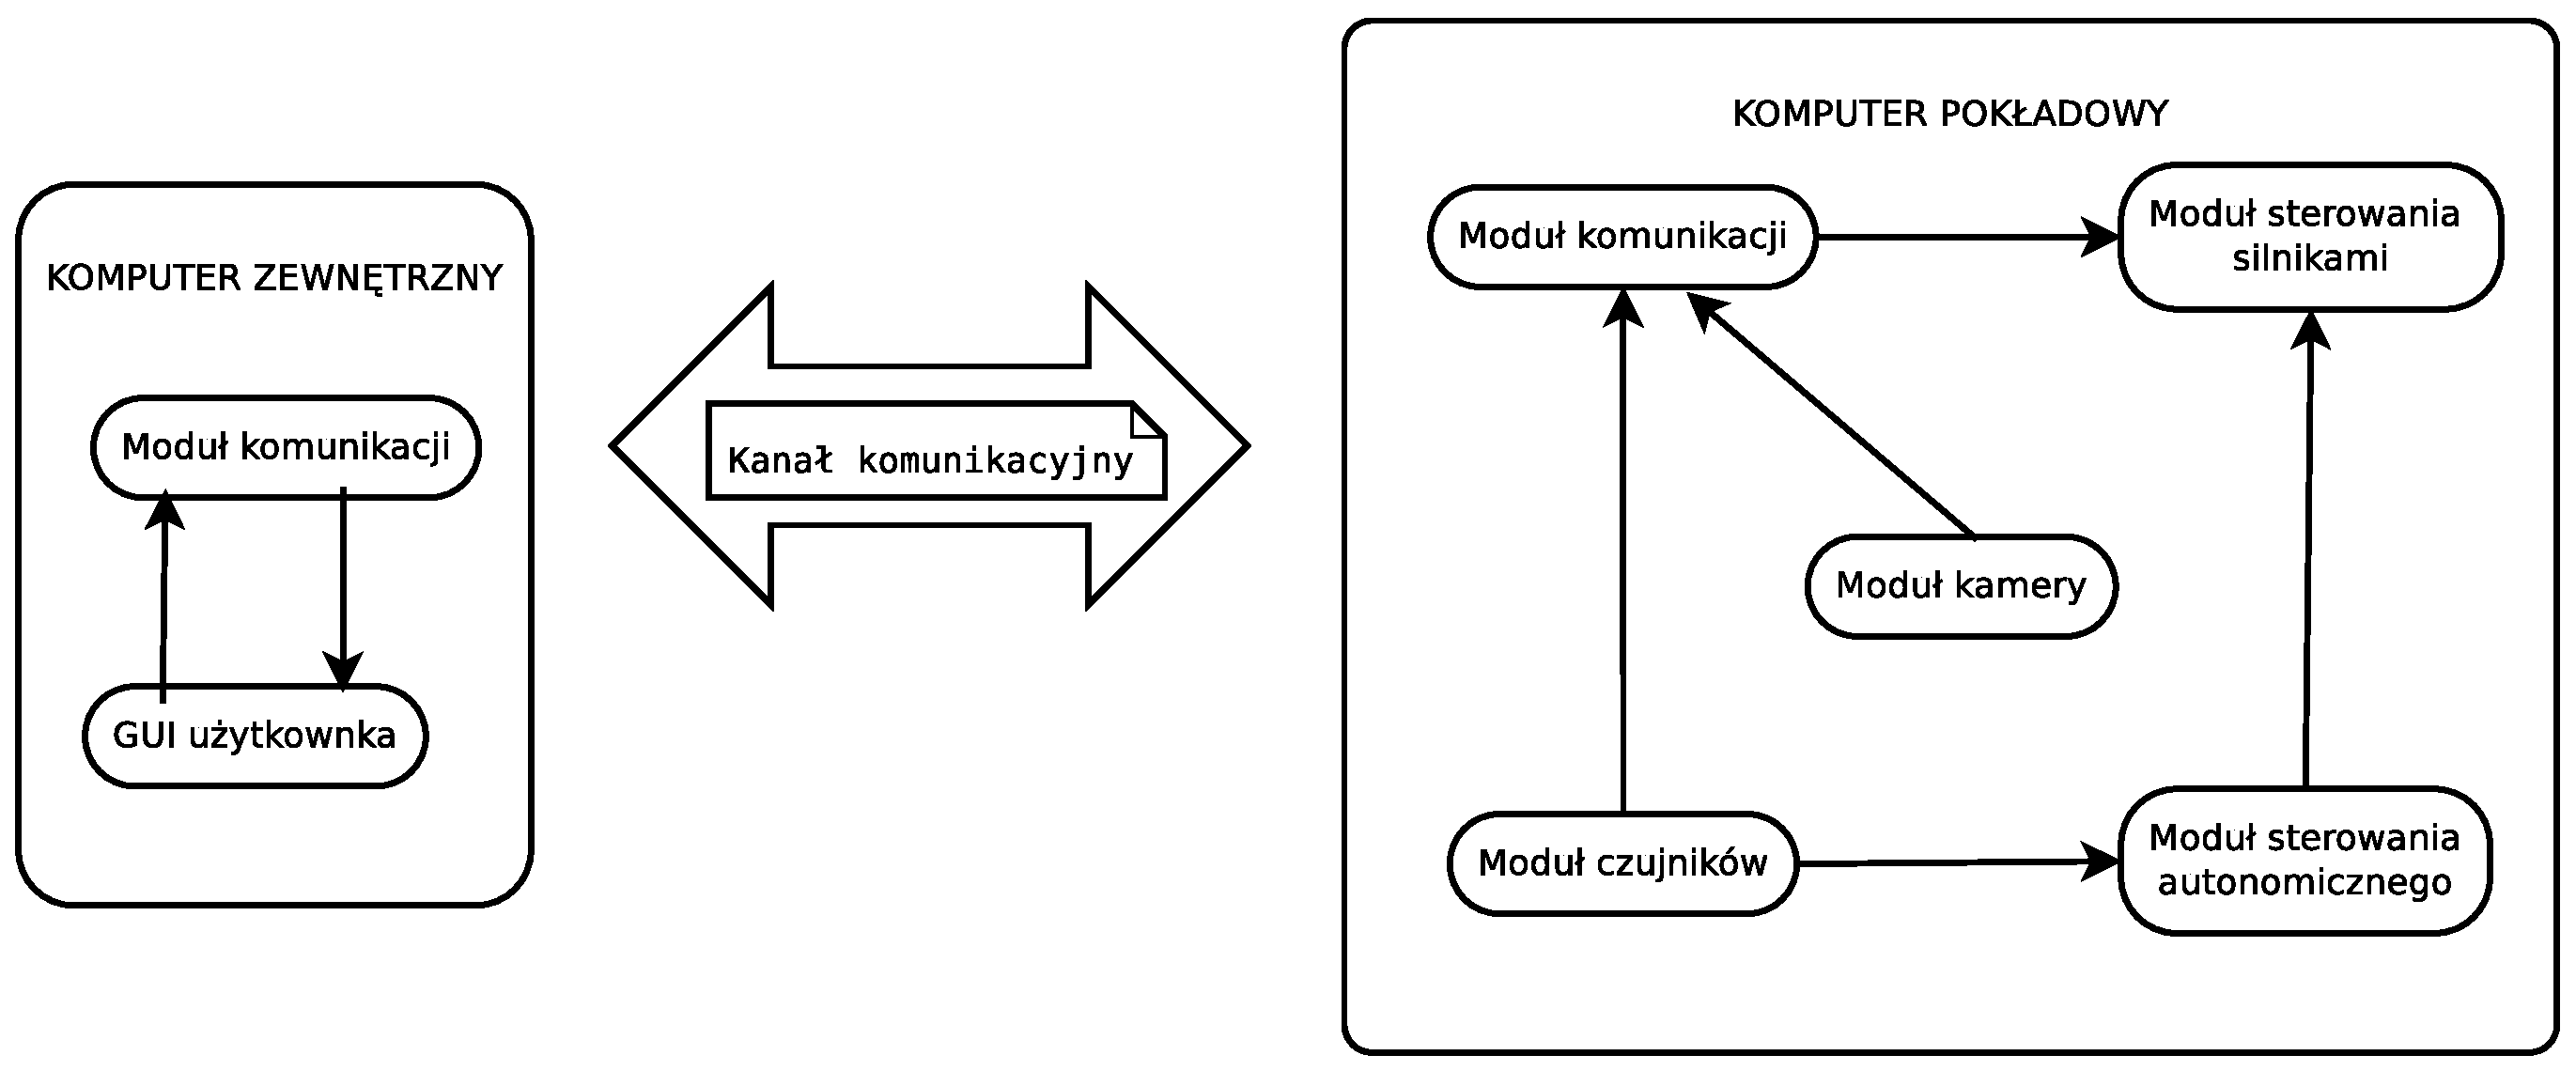
\includegraphics[width=15cm]{idea_programowa.eps}
\end{figure}

\section{Opis komponentów:}

\section{ Zależnosci we/wy:}

\section{ Kryteria ewaluacji:}

Robot czterokołowy umożliwi zdalne sterowanie w pomieszczeniu zamkniętym i dokonanie inspekcji pomieszczenia z zapisem video i sygnałów ze wszystkich czujników pomiarowych. Wykrywanie przeszkód odbywa się dwustopniowo: przez analizę danych z czujników ultradźwiękowych, oraz przez analizę danych odebranych z czujników stykowych. Po wykryciu przeszkody robot spróbuje ominąć przeszkodę. W razie braku możliwosci ominięcia przeszkody robot zatrzyma się.

\section{ Baza sprzętowa i programowa:}
Komputer pokładowy:
\begin{itemize}
\item Płytka uruchomieniowa: Raspberry Pi 1 model A
\item System operacyjny:     Raspbian GNU/Linux 8.0 (jessie)
\item Kompilator:            gcc 4.9.2
\item Framework robotyczny:  ROS indigo 1.11.16
\end{itemize}

Komputer zewnętrzny:
\begin{itemize}
\item System operacyjny:     Ubuntu 14.04.4 LTS (trusty)
\item Kompilator:            gcc 4.8
\item Framework robotyczny:  ROS indigo 1.11.16
\end{itemize}


\end{document}